\documentclass[]{article}

\usepackage[utf8]{inputenc}
\usepackage[english,serbian]{babel}
\usepackage[margin=0.7in]{geometry}
\usepackage{url}
\usepackage{float}
\usepackage[graphicx]{realboxes}
\usepackage{listings}
\usepackage{textcomp}
\usepackage{xcolor}
\usepackage{titlesec}
\usepackage{adjustbox}
\lstset {
    language=HTML,
    frame=none,
    %xleftmargin=-.25in,
    %xrightmargin=.25in
    framesep=10pt,
    tabsize=4,
    showstringspaces=false,
    upquote=true,
    commentstyle=\color{black},
    keywordstyle=\color{black},
    stringstyle=\color{black},
    basicstyle=\small\ttfamily,
    emph={int,char,double,float,unsigned,void,bool},
    emphstyle={\color{black}},
    escapechar=\&,
    classoffset=1,
    morekeywords={>,<,.,;,,,-,!,=,~},
    keywordstyle=\color{black},
    classoffset=0,
    breaklines=true
}
\pagenumbering{gobble}

\titlespacing\title{left spacing}{before spacing}{after spacing}[right]

\title{Ra\v{c}unarske mre\v{z}e 4R, Ispit - Septembar 2}
\date{22.09.2019.}

\begin{document}

\makeatletter
\begin{center}

{\fontsize{12pt}{14pt}\selectfont\bfseries\@title\par}
\@date
\vspace{5mm}

Pro\v{c}itati sve zadatke \textbf{pa\v{z}ljivo} pre rada - sve \v{s}to nije navedeno ne mora da se implementira! 

Na \texttt{Desktop}-u napraviti folder sa imenom u formatu \texttt{rm\_sept2\_Ime\_Prezime\_miGGXXX} i u njega smestiti \texttt{Java} projekat sa resenjima zadataka u zasebnim paketima sa imenima \texttt{zad1}, \texttt{zad2} itd. 

Vreme za rad: \textbf{2.5h}. Sre\'{c}no!
\end{center}
\makeatother


\begin{enumerate}
  \item Sockets \textbf{(15p)}
  \begin{itemize}
    \item Napraviti Java aplikaciju koja ima ulogu pojednostavljenog sistema za deljenje fajlova. Povezati se na lokalni server na portu 34567 koriste\'c{}i \texttt{Socket} klasu. Prilikom startovanja klijenta se bira re\v{z}im rada koji mo\v{z}e biti:
    \begin{itemize}
      \item \emph{send} - serveru se \v{s}alje fajl na putanji koja se unosi sa standardnog ulaza
      \item \emph{recv} - \v{c}eka se na pristizanje fajla od strane drugog klijenta, pri \v{c}emu se sadr\v{z}aj pristiglog fajla ispisuje na standardni izlaz
    \end{itemize} 
    Nakon biranja re\v{z}ima rada, klijent serveru \v{s}alje indikator re\v{z}ima (proizvoljno implementirati) i zatim izvr\v{s}ava akciju specifi\v{c}nu za izabrani re\v{z}im rada. \hfill (4p)
    \item Napraviti Java aplikaciju koja ima ulogu pojednostavljenog servera sistema za deljenje fajlova. Pokrenuti lokalni server na portu 34567 koriste\'c{}i \texttt{ServerSocket} klasu. Prilikom povezivanja na server svaki klijent se obradjuje u \textbf{zasebnoj niti}. \hfill (2p)
    \item Od klijenta se prima indikator re\v{z}ima rada i na osnovu njega se klijent obradjuje na odgovaraju\'c{}i na\v{c}in:
    \begin{itemize} 
      \item \emph{send} - prima se fajl od klijenta i prosledjuje klijentima u listi \v{c}ekanja, nakon \v{c}ega se svim klijentima zatvara veza \hfill (4p)
      \item \emph{recv} - klijent se sme\v{s}ta u listu \v{c}ekanja (proivoljno implementirati) dok ne primi fajl \hfill (4p)
    \end{itemize}
    \item Kako ne bi doslo do konflikata, ograni\v{c}iti da najvi\v{s}e jedan klijent mo\v{z}e biti u re\v{z}imu \emph{send} u isto vreme. Prilikom slanja re\v{z}ima rada serveru, ako ve\'c{} postoji klijent sa istim re\v{z}imom, prekinuti konekciju na serverskoj strani. \hfill (1p)
  \end{itemize}

  \item Swing \textbf{(15p)}
  \begin{itemize}
    \item Napraviti prozor i u njega dodati skrolabilnu komponentu za prikaz HTML sadr\v{z}aja. \hfill (2p)
    \item Dodati oblast za unos URL-a koji vodi do HTML fajla na lokalnom fajlsistemu. Dodati dugme \texttt{Prikazi} koje prikazuje sadr\v{z}aj tog HTML fajla u komponenti za prikaz. \hfill (2p)
    \item Omogu\'c{}iti da se prozor mo\v{z}e pro\v{s}iriti i smanjiti a da se raspored i razmera komponenti ne promeni. \hfill (3p)
    \item Dodati dugme \texttt{Sadrzaj} \v{c}iji je efekat da kreira HTML listu naslova iz HTML sadr\v{z}aja komponente za prikaz. Uvu\'c{}i svaki naslov onoliko puta koliki je njegov nivo (npr. \texttt{<h3>} naslov se uvla\v{c}i 3 puta). Prikazati kreirani HTML u komponenti za prikaz. \hfill (5p)
    \item Podvu\'c{}i sve naslove koji su nivoa $1$. \hfill (1p)
    \item Ispo\v{s}tovati izgled aplikacije (ne me\v{s}ati redosled komponenti i postarati se da su odnosi u veli\v{c}ini kao na slici na narednoj strani). \hfill (2p)
    \item Omogu\'c{}iti da se prozor mo\v{z}e pro\v{s}iriti i smanjiti a da se raspored i razmera komponenti ne promeni. \hfill (2p)
  \end{itemize}

\end{enumerate}


\newpage

\begin{figure}[H]
  \centering
  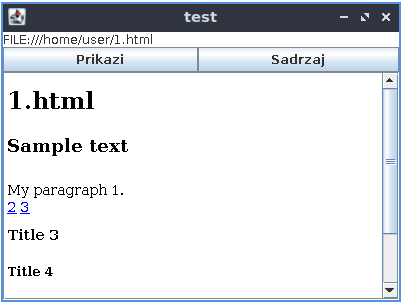
\includegraphics[scale=0.7]{fig1.PNG}
  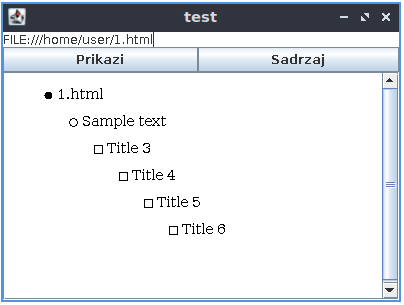
\includegraphics[scale=0.7]{fig2.PNG}
  \label{fig2}
  \caption{Izgled aplikacije pre i posle aktivacije dugmeta \texttt{Sadrzaj}}
\end{figure}


HTML test fajlovi:\\

\noindent
\begin{tabular}{ccc}
\begin{lstlisting}
  <!DOCTYPE html>
  <html>
    <body>
      <h1>1.html</h1>
      <h2>Sample text</h2>
      
      <p>My paragraph 1.</p>

      <a href="2.html">2</a>
      <a href="3.html">3</a>

      <h3>Title 3</h3>
      <h4>Title 4</h4>
      <h5>Title 5</h5>
      <h6>Title 6</h6>

      Some text goes here.
    </body>
  </html>
\end{lstlisting}&
\begin{lstlisting}
  <!DOCTYPE html>
  <html>
    <body>
      <h1>2.html</h1>
      <h2>Sample text</h2>
      
      <p>My paragraph 2.</p>

      <a href="1.html">1</a>
      <a href="3.html">3</a>

      <h2>Title 2</h2>
      <h1>Title 1</h1>
      <h5>Title 5</h5>
      <h4>Title 4</h4>

      Text text text text.
    </body>
  </html>
\end{lstlisting}&
\begin{lstlisting}
  <!DOCTYPE html>
  <html>
    <body>
      <h1>3.html</h1>
      <h2>Sample text</h2>
      
      <p>My paragraph 3.</p>

      <a href="1.html" 
          id="1">1</a>
      <a href="2.html" 
          class="2">2</a>

      <h4>Title 4</h4>
      <h5>Title 5</h5>
      <h6>Title 6</h6>
      <h2>Title 2</h2>

      Text text text text.
    </body>
  </html>
\end{lstlisting}
\end{tabular} 

\end{document}
